\documentclass{homework}
% \usepackage{graphicx} % Required for inserting images
\usepackage{amsmath}
\usepackage{gensymb}
\usepackage{subfig}
\usepackage{float}

\class{ECEN 5427}
\title{Homework 3}
\author{Sean Jennings}
\date{April 21, 2025}

\begin{document}
\maketitle

\newcommand{\G}{\mathcal{G}}
\newcommand{\T}{\mathcal{T}}
\newcommand{\coal}{\text{coal}}
\newcommand{\nuclear}{\text{nuclear}}
\newcommand{\wind}{\text{wind}}
\newcommand{\solar}{\text{solar}}
\newcommand{\gas}{\text{gas-cc}}

\section{Part 1: Problem Formulation}
\begin{enumerate}
\item Let $\G = \{\coal, \gas, \nuclear, \solar, \wind\}$ be the set of all generation types
available. Let $\T = [1, 2, \dots, 8760]$ be the set of hourly timesteps throughout the year. These
are the sets over which our decision variables (and some parameters) vary.

The parameters of the model are the variables which are input to the model. For each generation type $g \in \G$
and each timestep $t \in \T$, let $\eta_{g, t}$ be the capacity factor of $g$ at time $t$. Note that for each 
dispatchable generation type $g \in \mathcal{D} = \{\coal, \gas, \nuclear\}$, we have $\eta_{g,t} = 1$ for
all $t \in \T$.

For each timestep $t\in \T$, let $\lambda_t$ be the system load (in MW) at time $t$. Both $\eta$ and $\lambda$
are given in timeseries.csv.

To compare capital and operational costs, we will assume a plant lifetime $L_g$ (in years) for each generation type $g\in\G$,
and then annualize capital costs over the lifetime of the plant.

Let cost $C_{0,g}$ per unit of installed (in \$/MW)
and $C_{1,g}$ be the cost per unit of energy generated in (\$/MWh) for a given generator $g\in\G$.
$C_{0,g}$ is calculated from the capital costs $C_{cap,g}$ and fixed O\&M costs $C_{FOM,g}$ (scaling units appropriately) via the relation
\begin{equation*}
    C_{0,g} = C_{cap,g} / L_g + C_{FOM,g}
\end{equation*}
and $C_{1,g}$ is the sum of variable O\&M cost and fuel cost. All costs are taken from the
given file plant\_characteristics.csv.

Specifically, we'll take $L_{\text{nuclear}} = 50$, $L_{\text{gas-cc}} = L_{\text{coal}} = 40$, and $L_{\text{wind}} = L_{\text{solar}} = 25$.

In summary, our parameters are $\eta$, $\lambda$, $C_0$ and $C_1$. 
(We drop the subscripts to denote the full vector/matrix across all members of pertinent sets.)

\item To solve the greenfield capacity expansion problem, we must determine the amount of capacity to install
for each generation type. For each $g\in \G$, let $x_g$ be the amount of capacity installed (in MW) for generation
type $g$.

The generation mix must be able to meet load at each timestep. Therefore, our optimization formuation must
simultaneously search for a feasible dispatch. For each $g\in\G$ and $t \in \T$, let $p_{g, t}$ be the power
output (in MW) of generation type $g$ at time $t$.

$x$ and $p$ are the decision variables.

\item Our objective is to minimize total system costs, including both capital and operational costs. For simplicity,
we'll assume 0\% interest rates and annualize the capital costs over the lifetime of each generation type. We'll
let the function $f$ denote the cost function, representing yearly cost as a function of installed capacity $x$ and dispatch $p$, given by
\begin{equation*}
    f(x, p) = \sum_{g\in\G} \biggl[C_{0, g} x_g + C_{1,g} \sum_{t\in\T} \Delta t \cdot p_{g,t} \biggr]
\end{equation*}
where $\Delta t = 1$ [hr] is the length of each timestep.

\item Our first constraint is on our dispatch $p_{g,t}$, which is limited by the installed capacity $x_g$ and capacity factor $\eta_{g,t}$
by the inequalities
\begin{equation*}
    0 \leq p_{g,t} \leq \eta_{g,t} \cdot x_g \qquad (\forall g\in\G, t\in\T).
\end{equation*}

Our second constraint is that the sum of dispatch must equal load at each timestep. I.e.
\begin{equation*}
    \sum_{g\in\G} p_{g,t} = \lambda_t \qquad {\forall t\in\T}
\end{equation*}

Thus, our full capacity expansion problem is given by:
\begin{align*}
     \min_{x, p} &\qquad f(x, p) \\
    \text{subject to:}  &\qquad
    0 \leq p_{g,t} \leq x_g & (\forall g\in\G, t\in\T) \\
    &\qquad \sum_{g\in\G} p_{g,t} = \lambda_t &(\forall t\in\T)
\end{align*}


\section{Part 2}

\item Numerical results of the JuMP implementation of the optimization are shown in table
\ref{tab:objective}.
We tabulate the optimal objective value and optimal generation levels across a
few different parameter inputs.

Upon first implementation, I implicitly assumed a lifetime of 1 year for each plant
(i.e. $L_g = 1$ for all $g\in\G$). I've left this result in, since it is an interested
limit case (as discussed in question 7).

\begin{center}
    
\begin{tabular}{rrrrrr}
    \hline
     & $L_g=1$ & Base Case
        & $\epsilon_{max}$ = 100.0
        & $\epsilon_{max}$ = 10.0 & $\epsilon_{max}$ = 0.0 \\
    \hline
    objective (billion \$) & 164.213 & 18.8918 & 18.8918 & 19.6929 & 24.107 \\
    coal (GW) & 0.0 & 0.597322 & 0.59432 & 0.0 & 0.0 \\
    gas-cc (GW) & 73.651 & 35.3762 & 35.3792 & 24.475 & 0.0 \\
    nuclear (GW) & 0.0 & 34.7877 & 34.7877 & 46.2384 & 70.7279 \\
    solar (GW) & 0.0 & 4.45751 & 4.45751 & 5.51959 & 5.25622 \\
    wind (GW) & 0.0 & 2.53293 & 2.53293 & 1.03264 & 1.18098 \\\hline
\end{tabular}
    \captionof{table}{
        Objective values and installed capacity across a few different model inputs.
        Note: the units for all $\epsilon_{max}$ values are million tonnes.
    }
    \label{tab:objective}
\end{center}


The objective value is $1.8989 \times 10^{10}$. This indicates the total annualized cost in dollars.
Note that in the table we divide by $10^9$ to display in the more human-friendly unit of billions
of dollars (and likewise capacities are converted to GW).

\item The capacities in table \ref{tab:objective} show that the majority of the total capacity
is met by a combination of nuclear and natural gas. Table \ref{tab:costs} shows the values of $C_0$
and $C_1$ across generation types, which allows us to compare how fixed and marginal
costs vary. Nuclear has higher fixed costs, but lower marginal costs than combined-cycle
natural gas, so the optimization finds it is more cost effective to fulfill the base load
with nuclear (a high capacity factor makes up for high capital costs) and peak loads
with natural gas (where as a result of lower capacity factors, marginal costs play less of a role).

\begin{center}
\begin{tabular}{rrr}
    \hline
    \textbf{Generation Type} & \textbf{C0 (\$/kW)} & \textbf{C1 (\$/MWh)} \\
    \hline
    coal & 147.0 & 28 \\
    gas-cc & 77.0 & 38 \\
    nuclear & 285.0 & 9 \\
    solar & 79.0 & 0 \\
    wind & 95.0 & 0 \\\hline
\end{tabular}
    \captionof{table}{Costs for different generation types}
    \label{tab:costs}
    
\end{center}



As seen in table \ref{tab:objective}, marginal costs for coal are only slightly lower than gas-cc, but with nearly
twice the capital cost. Thus, coal is only utilized for a narrow shoulder between base and peak loads.

While wind and solar have zero marginal cost and capital costs that are on par with natural gas,
they contribute less to the generation mix. This can be explained by their limited capacity factor
as well as the temporal misalignment between renewable availability and load. If even one day
(or a single hour!) has a high load and low renewable availability, meeting the low will be
impossible with a renewable-heavy system.

Figure \ref{fig:dispatch} shows a plot of the dispatch stack on the day which load peaks, illustrating the points
made above.

\begin{center}
    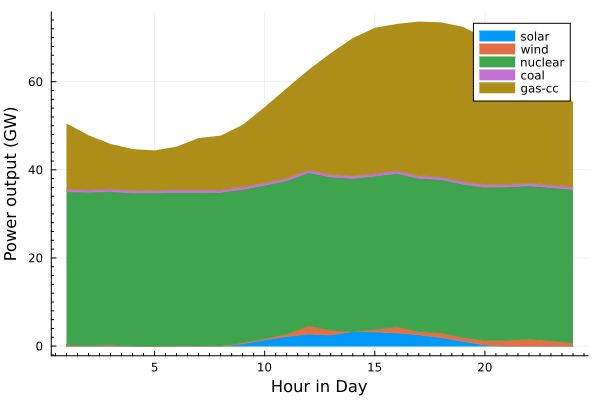
\includegraphics[width=0.8\linewidth]{Images/dispatch_stack.png}
    \captionof{figure}{Dispatch Stack on Peak Day (Base Case)}
    \label{fig:dispatch}
\end{center}

\item
\begin{letterenum}
\item 
To capture the emissions limit, we introduce the parameters $\epsilon_{g}$,
representing the emissions factor for each generation technology, with units
(metric tonnes CO$_2$)/MWh, and $\epsilon_{max}$ representing the emissions constraint.
We then add the constraint that total emissions (the sum of generation weighted by emissions factor)
must be less than the prescribed value:
\begin{equation*}
    \sum_{t\in\T} \biggl[ \Delta t \sum_{g\in\G} \epsilon_g p_{g,t} \biggr] \leq \epsilon_{max}
\end{equation*}

\item Table \ref{tab:objective} shows the emission-constrained results next to the original ones. We find
that the original generation mix already satisfies the suggested $\epsilon_{max}=$100 million
metric ton limit. We also compute optimal generation mixes for more stringent limits.


With $\epsilon_{max}=10$ million tonnes CO$_2$, the coal generation is entirely retired and natural
gas generation is reduced by a sizable 10 GW. Interestingly, it is replaced by primarily by
nuclear generation. Solar generation increases by about a GW, while wind is reduced
by 1.5 GW. Again, this is due to the fact that renewables are not necessarily available when the system peaks.
This puts a lower bound on the amount of dispatchable resources required. With capital already
invested in dispatchable plants, only a relatively small amount of wind and solar can be justified.

\end{letterenum}

\item The most surprising part of the analysis to me was the initial result with $L_g = 1$ year
for all $g\in\G$,
where the generation is entirely filled by natural gas. But there is a simple explanation:
comparing the entire capital costs against only a year's worth of O\&M costs heavily weighs
capital costs over marginal ones. Since gas-cc is dispatchable and requires relatively little
capital, it makes sense that it is favored over all else.

After introducing more realistic lifetimes, the results make intuitive sense to me, for
the reasons already explained. Since we neglect the possibility of energy storage, 
dispatchable (firm) resources are favored over variable ones. The emissions constraint
works as intended, entirely eliminating coal and gas-cc in the case of zero allowed emissions.

To make the analysis more realistic, the first thing that comes to mind is energy storage.
Energy storage (at a reasonable cost) would help "firm" the wind and solar resources,
shifting them to cover peak loads and unlocking their zero-marginal benefits.

Beyond storage, there are a plethora of additional considerations which would make the modeling
more realistic, including (but not limited to) ancilliary reserves, dynamic stability constraints,
and ramping constraints.



\end{enumerate}










\end{document}
